\dev{Emile Martinez}{}{}{}

\begin{com}
	Comme il y a beaucoup à dire, et que le titre ne mentionne pas d'aspects théoriques sur les structures, on suppose ici les structures déjà définie dans le cours. Ainsi, on rappelera uniquement, pour uniformisation les méthodes caractéristiques. On se concentre ainsi sur les implémentations et les applications.
\end{com}

\subsection{Les piles}

\textbf{Rappel :} Une pile est une structure de données avec les méthodes \texttt{vide}, \texttt{est\_vide}, \texttt{empiler}, \texttt{depiler}.

\subsubsection{Implémentation par listes}

Cette manière est immédiate et donc naturelle.

\begin{exercise}[Au tableau avec participation des élèves]
	A quoi correspondent les opérations de bases de la pile sur une liste (à l'oral et éventuellement avec le dessin d'une liste simplement chaînés pour montrer les modifications).
\end{exercise}

Les listes étant naturelles en OCaml, nous les implémenterons de cette manière en Ocaml. Néanmoins cette pile est immuable.

\subsubsection{Implémentation par tableaux}

La deuxième manière est en utilisant un tableau. \\

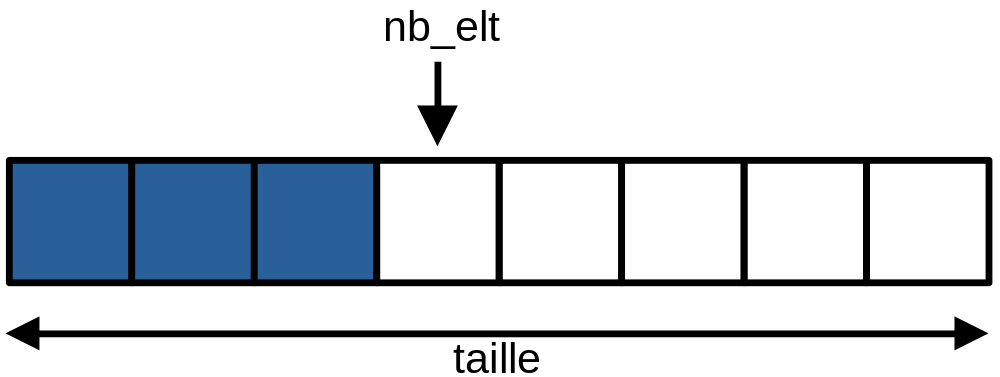
\includegraphics[scale=0.3]{lecon/05-piles_files/piles_tableau.png}
\\

\begin{idee}
	Pour cela, on utilise un indice \texttt{nb\_elt} qui nous indiquera à quelle case du tableau correspond le sommet de la pile, les cases précédentes du tableau contenant les autres éléments empilés.
\end{idee}


\begin{impl}
	On doit soit alors utiliser un tableau de taille fixe (et donc connaître à l'avance le nombre max d'éléments dans la pile)
\end{impl}


\begin{exercise}
	Quels sont les inconvénients de cette implémentation ? ( le fait qu'il faut soit utilisé un tableau dynamique, soit connaître à l'avance la taille maximale de la pile)
\end{exercise}

\begin{impl}
	en C en TP avec les déclarations déjà faites, \texttt{vide} également, et le corps des autres fonctions à remplir
\end{impl}


\begin{rem}
	Les problèmes sont exactement similaires à ceux de l'implémentation d'une liste par un tableau. Cela vient de la proximité entre une liste et une pile.
\end{rem}

\begin{exercise}
	Laquelle de ces deux implémentations est mutable ? Immuable ?
\end{exercise}

\subsubsection{Complexité}

Toutes ces opérations sont en $O(1)$. De plus sa complexité spatiale n'est, si l'implémentation est bien effectuée, que O(hauteur maximale de la pile)

\subsection{Les files}

\textbf{Rappel :} Une file est une structure de données avec les méthodes \texttt{vide}, \texttt{est\_vide}, \texttt{enfiler}, \texttt{defiler}.

\subsubsection{Par une liste chaînée}

\begin{idee}
	On stocke les entrées dans une liste et on à l'aide de pointeurs le début et la fin de la file.
\end{idee}

\begin{center}
	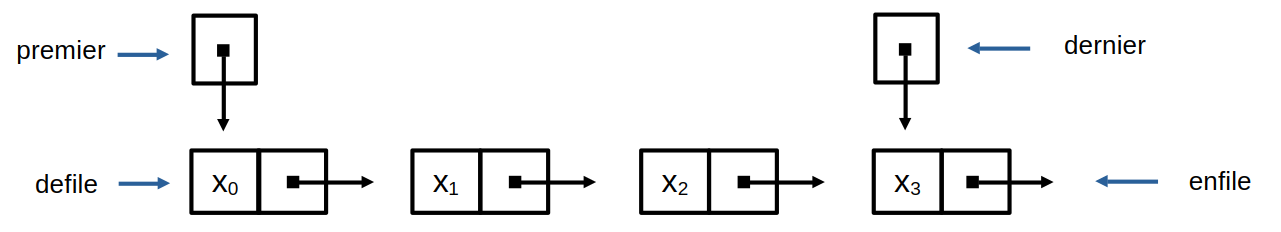
\includegraphics[width=0.8\linewidth ]{lecon/05-piles_files/liste_chainee.png}
\end{center}

\begin{impl}
	Ainsi, ajouter des éléments consiste seulement à enlever l'élément du début et à passer début sur l'élément suivant de la liste et enlever un élément consiste simplement à ajouter un élément à la fin de la liste et à y faire pointer le pointeur fin.
\end{impl}

\begin{exercise}
	Quelle est l'intérêt des pointeurs fin et début ?(fin pour trouver la fin de la liste en O(1), début pour repérer la liste, équivalent à garder le premier élément de la file)
\end{exercise}

\begin{exercise}
	Comment encode-t-on la file vide ?
\end{exercise}


\subsubsection{Par un tableau}

\begin{idee}
	Les éléments sont stockés consécutivement dans un tableau avec deux indices début et fin indiquant dans le tableau le début de la liste et la fin de la liste.
\end{idee}

\begin{exercise}
	Quelle est la complexité de chaque opération élémentaire ?
\end{exercise}

\textbf{Problème :} La complexité spatiale est en O(nombre de \texttt{enfile}) alors que l'on souhaiterait avoir O(longueur maximale de la file)

\begin{idee}
	Pour cela, si l'on connaît à l'avance une borne sur cette longueur maximale, on peut utiliser des indices modulo cette borne (et ainsi utilisé un tableau «circulaire»)
\end{idee}

\begin{center}
	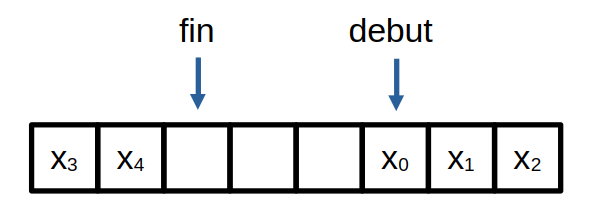
\includegraphics[width=0.45\linewidth ]{lecon/05-piles_files/tableau_circulaire.png}
\end{center}


Ces deux implémentations sont mutables.

\subsubsection{Par deux listes mais de manière immuable}


\begin{idee}
	Il est possible de créer efficacement une telle structure en utilisant uniquement deux piles : 
	\begin{itemize}
		\item La première contiendra les éléments prêts à sortir
		\item La deuxième contiendra les éléments que l'on vient de rajouter
	\end{itemize}
\end{idee}


\begin{rem} 
	En choississant efficacement quand on les fait passer de l'un à l'autre, on peut avoir une structure efficace.
\end{rem}


\begin{proposition}
	Il existe une implémentation de la structure de file pour laquelle la complxité temporelle de chaque opération est en O(1) amorti
\end{proposition}


\textbf{Développement} Implémentation d'une file PAPS avec deux listes et (au choix) introduction à la complexité amortie / implémentation par une liste doublement chaînées

\subsubsection{Pour aller plus loin}

Une liste doublement chaînée peut, au pris d'une lourdeur relative dans l'implémentation, fournir immédiatement les opérations de la pile et de la file combinée en O(1)

\subsection{File de priorité}

\textbf{Rappel :} Une file de priorité est une structure de donnée ayant les méthodes \texttt{vide}, \texttt{est\_vide}, \texttt{insérer}, \texttt{extraire\_min}

\subsubsection{En théorie}

\begin{idee} 
	Nous implémenterons les files de priorité à l'aide de tas min.
\end{idee}

\begin{definition}
	Un tas min est un arbre binaire presque complet où chaque noeud à un attribut plus petit que ceux de ses fils
\end{definition}

\paragraph{L'insertion}
	On ajoute l'élément à l'endroit au seul endroit qui préserve la structure de tas (petit dessin).
	
	Ensuite, on l'inverse successivement avec son père, si il est plus petit que lui.

	\begin{theorem}
		cet algorithme préserve la structure de tas min
	\end{theorem}

\paragraph{Récupérer l'élément minimum}

	On enlève la racine, on prend le dernier élément du tas, on le met à la position de la racine, et tant qu'un fils est plus petit que lui, on l'échange avec son fils le plus petit.

	\begin{theorem}
		Cet algorithme préserve la structure de tas.
	\end{theorem}
\enspace \\
\begin{theorem}
	Toutes ces opérations sont en $O(\log(n))$ où $\log(n)$ est le nombre d'éléments dans le tas.
\end{theorem}

\begin{com}
	Cette application n'est pas avec les autres car assez immédiate
\end{com}

\begin{appl}
	Tri par tas en $O(n \log(n))$
\end{appl}

\subsubsection{En pratique}

\begin{idee} 
	Pour implémenter de tels arbres, on peut les implémenter comme des structures récursives, en gardant le chemin jusqu'à la dernière feuille sous forme de listes de droite/gauche
\end{idee}

\begin{exercise}
	Expliciter l'algorithme permettant de mettre à jour le chemin
\end{exercise}

\begin{com}
	C'est un algorithme d'addition binaire, où quand on doit rajouter un 1 (droite), on rajoute un 0 (gauche). Donc c'est cet algorithme avec 111+1 = 0000 et 0000-1 = 111 (et le nombre de 0 qui importe)
\end{com}

\begin{exercise}
	Implémenter cette structure en OcamL
\end{exercise}

\begin{idee}
	Sinon, on peut l'implémenter comme un tableau où le fils de l'élément à l'indice i, sont stockés aux indices $2i+1$ et $2i+2$.
\end{idee}

\begin{exercise}
	Faire cette implémentation en C
\end{exercise}

\subsection{Applications aux graphes}

\begin{algorithm}[H]
	\caption{Parcours de graphe}
	$a\_faire \gets vide()$ \\
	$a\_faire.ajouter(s0)$ \\
	\Tq{$a\_faire$ n'est pas vide}{
		$u \gets a\_faire.extraire()$\\
		\Si{$u$ n'a pas encore était visité}{
			\Pour{$v$ voisin de $u$}
			{
				$a\_faire.ajouter(v)$
			}
		}
	}
\end{algorithm}

Si $a\_faire$ est une pile, on fait un parcours en profondeur et si $a\_faire$ est une file PAPS, on fait un parcours en largeur.

\begin{algo}[Algorithme de Djikstra]
	\enspace \\
	On cherche la distance dans un graphe pondéré d'un sommet s à chaque autre sommet.\\
	\\
	On fait le parcours de graphe avec une file de priorité pour $a\_faire$. On garde un tableau des distances, que l'on met à jour à chaque étape. La priorité dans la file est la distance que l'on a au moment de l'insertion, et on ajoute toujours les voisins non encore visité.\\
	\\
	On obtient alors les plus courts chemins.
\end{algo}

\subsection{Applications systèmes}

Ces structures sont utilisés dans de nombreuses applications à bas niveau.

\subsubsection{Pile d'appel}

Quand on exécute un programme avec des appels successifs à des fonctions, de nouvelles variables sont crées, des emplacements pour les arguments, etc..., mais à la fin de la fonction, on doit restaurer l'environnement précédent.

\begin{idee}
	Pour cela, à chaque appel de fonctions, on empile l'état actuel sur une pile, et à chaque retour de fonction, on restaure l'état au sommet de la pile (que l'on dépile).
\end{idee}

\begin{com}
	Suivant la place (notamment si on ne prend pas tous les exemples), on peut rajouter un schéma
\end{com}

\subsubsection{Ordonnancement}

    Pour gérer le parrallélisme, un ordonnanceur doit décider, quel processus doit être executé.

Pour cela on peut par exemple : \begin{itemize}
	\item stocker les processsus dans une file de priorité pour que les processus les plus importants soient executés en premier.
\begin{example} avec comme clé, la date butoire de fin d'éxecution, on exécute en premier les plus urgents
\end{example}
	\item Mettre les processus dans une file, en prendre le premier élément, l'exécuté pendant un certain temps, puis le remettre en queue de file. C'est l'algorithme du tourniquet, qui garantie que tous les processus s'exécuterons un jour.
\end{itemize}

\subsubsection{Tampon}
	
	Dès que l'on a deux programmes dont la sortie de l'un est branché sur l'entrée de l'autre, et qui ne travaille pas à la même vitesse, on doit mettre un tampon entre les deux. On utilise alors une file PAPS pour stocker les données en attendant que le deuxième programme les récupère.
	
	\begin{example}
		On reçoit des paquets du réseau. On doit les récupérer. On les mets dans un tampon, le temps que le programme viennent les traiter. On les restiture alors dans l'ordre d'arrivée grâce à la file.
	\end{example}

\begin{com}
	Par manque de place, on peut éventuellement passer sur certains exemples, et eventuellement rajouter plein de schéma un peu partout dans la leçon. De plus, on peut évoquer à l'oral la vraie application dans un cours, surtout pour les piles et les files, qui seraient l'application pédagogique d'illustrer la différence type abstrait et structure sous-jacente, et donc ce que sont les méthodes sur les structures et la modularité de tout cela.
\end{com}